
% !TEX program = xelatex
\documentclass[12pt,a4paper]{report}

% ---------- PACKAGES ----------
\usepackage{fontspec}
\newfontfamily\azerbaijanifont{Times New Roman}

\usepackage{setspace}
\usepackage{geometry}
\usepackage{graphicx}
\usepackage{tikz}
\usetikzlibrary{arrows.meta, shapes, positioning, calc}
\usepackage{amsmath}
\usepackage{amssymb}
\usepackage[version=4]{mhchem}
\usepackage{titlesec}
\usepackage{booktabs}
\usepackage{array}
\usepackage{float}
\usepackage{multirow}
\usepackage{fancyhdr}
\usepackage{caption}
\usepackage{hyperref}
\usepackage{xcolor}

\usepackage[style=ieee,backend=biber,sorting=none,giveninits=true,url=false,isbn=false]{biblatex}
\addbibresource{references.bib}

\geometry{margin=1in}
\onehalfspacing
\setlength{\emergencystretch}{3em}

% ---------- HEADER ----------
\pagestyle{fancy}
\fancyhf{}
\fancyfoot[C]{\thepage}

% ---------- QUESTION STYLE ----------
\newcommand{\question}[1]{\par\noindent\textcolor{blue}{\textit{#1}}\par}
\newcommand{\answer}[1]{\noindent #1\par\vspace{0.6em}}
\newcommand{\coverlogo}[2]{%
  \IfFileExists{#1}{\includegraphics[width=#2\textwidth]{#1}}{\fbox{\parbox[c][2.5cm][c]{#2\textwidth}{\centering Logo placeholder}}}%
}

% ---------- DOCUMENT ----------
\begin{document}

% =========================
% COVER PAGE
% =========================
\begin{titlepage}
  \centering

  \vspace*{2cm}

  {\Large \textbf{Internship Report}}\\[1cm]

  {\Huge \textbf{Super-resolution for Fourier Transform Mass Spectrometry in the frequency domain}}\\[2cm]

  \textbf{Rajab İskandarli}\\[0.5cm]

  Computer Science\\[1cm]

  \textbf{Internship Period:} January 22 -- June 2\\[1cm]

  \textbf{Supervisors:}\\
  Dr. Christian Rolando\\
  Professor Pierre Collet\\
  Dr. Ulviyya Abdulkarimova

  \vfill

  \coverlogo{Logo UFAZ.png}{0.3}\hfill
  \coverlogo{cnrs_hauts_de_france_logo.jpg}{0.3}

  \vfill
\end{titlepage}

% =========================
% FRONT MATTER
% =========================
\pagenumbering{roman}

\chapter*{Abstract}
\addcontentsline{toc}{chapter}{Abstract}

\noindent\textbf{English:}\par
Fourier Transform Mass Spectrometry (FTMS) is widely used for high-resolution molecular analysis but is limited by acquisition time and frequency-domain resolution. The motivation for this project is to leverage deep learning-based super-resolution methods to enhance the spectral resolution without increasing measurement duration. By training neural networks on high- and low-resolution FTMS spectra, the model learns to reconstruct high-resolution frequency-domain signals from standard measurements. This approach allows better discrimination of closely spaced peaks, improves signal-to-noise ratios, and reduces spectral artifacts. The study evaluates the performance of several neural network architectures on both simulated and experimental datasets, comparing their ability to recover fine spectral features. Results indicate that deep learning super-resolution significantly enhances FTMS analytical precision, offering a scalable solution for complex molecular analysis in proteomics, metabolomics, and other applications.

\noindent\textbf{Azerbaijani:}\par
{\azerbaijanifont
  Fourier Transform Kütlə Spektrometriyası (FTMS) yüksək dəqiqlikli molekulyar analiz üçün geniş istifadə olunur, lakin əldə etmə müddəti və tezlik domeni üzrə qətnamə ilə məhdudlaşır. Bu layihənin məqsədi ölçmə müddətini artırmadan spektral qətnaməni yüksəltmək üçün dərin öyrənmə əsaslı super-qətnamə metodlarından istifadə etməkdir. Neyron şəbəkələr yüksək və aşağı qətnaməli FTMS spektrləri üzərində öyrədilərək standart ölçmələrdən yüksək qətnaməli tezlik domeni siqnallarını bərpa etməyi öyrənir. Bu yanaşma sıx yerləşmiş pikləri daha yaxşı ayırd etməyə, siqnal-səs nisbətini artırmağa və spektral artefaktları azaltmağa imkan verir. İş bir neçə neyron şəbəkə arxitekturasının simulyasiya edilmiş və eksperimental məlumat dəstlərindəki performansını qiymətləndirir və onların incə spektral xüsusiyyətləri bərpa etmək qabiliyyətini müqayisə edir. Nəticələr göstərir ki, dərin öyrənmə super-qətnaməsi FTMS analiz dəqiqliyini əhəmiyyətli dərəcədə artırır və proteomika, metabolomika və digər tətbiqlərdə mürəkkəb molekulyar analiz üçün miqyaslana bilən həll təqdim edir.
}

\chapter*{Acknowledgements}
\addcontentsline{toc}{chapter}{Acknowledgements}

\noindent I would like to express my sincere gratitude towards Dr. Ulviyya Abdulkarimova for believing in my capabilities and providing me an opportunity to carry out this internship.

\noindent I am most thankful to Dr. Christian Rolando for his supervision, expert guidance, and encouragement throughout the entire research process. His knowledge and critical remarks had a determining influence on the focus and quality of this research.

\noindent I also want to express special gratitude to Professor Pierre Collet for his continuous guidance and encouragement during the phases of the internship. His contribution enormously enhanced the technical level of the project.

\noindent I would also like to express my gratitude to the administrative and academic staff members at UFAZ for creating a welcoming, well-structured, and cooperative environment. Their organizational and educational support greatly assisted in the facilitation of my work during this internship.

\tableofcontents
\newpage

% =========================
% MAIN CONTENT
% =========================
\pagenumbering{arabic}

\chapter{Professional Environment}

\section{University of Lille and the MSAP UAR 3290 CNRS Laboratory}

The University of Lille is a major and top-ranked French public research institution. It
originates from the University of Douai, established in 1559, and assumed a contemporary form in 2018 through the union of the three previously independent universities of Lille 1 (Science and Technology), Lille 2 (Health and Law), and Lille 3 (Humanities and Social Sciences). Featuring a student and staff body of over 80,000 and 3,300 respectively, it is a central figure in European research and higher education. It is a University of Excellence since 2017 and was awarded a strategic endowment of €500 million to increase academic innovation, interdisciplinarity, and international openness.

The university is strongly embedded in the national French research environment, having established powerful partnerships with top research institutions like CNRS (Centre National de la Recherche Scientifique), INSERM (Institut National de la Santé et de la Recherche Médicale), INRIA (National Institute for Research in Digital Science and Technology), INRAE (National Research Institute for Agriculture, Food and Environment), and CHU Lille (Lille University Hospital). It is also closely tied to top-flight engineering and policy schools like École Centrale de Lille and Sciences Po Lille, enabling cross-disciplinary learning and applied research.

% \begin{figure}[h]
% \centering
% \includegraphics[width=0.7\textwidth]{msap_lab.png}
% \caption{UAR 3290 MSAP Laboratory}
% \end{figure}

Housed in this dynamic setting, the MSAP UAR 3290 (Miniaturization for Synthesis, Analysis, and Proteomics) is a research facility with a high degree of specialization under the umbrella of the CNRS. Formed in January 2010 and headed by Professor Ahmed Mazzah, MSAP is a Support and Research Unit (Unité d’Appui et de Recherche) that connects fundamental scientific research with applied analytical technology.

Its mission is to promote innovative methods in mass spectrometry, chromatographic separation, proteomics, and physical-organic chemistry. MSAP is also part of major infrastructures such as Infranalytics (France), IPERION HS, and E-RIHS (Europe), and plays a key role in biological and heritage science research.

The laboratory is organized into three scientific axes:

\begin{itemize}
  \item \textbf{Instrumental Development:} led by Dr. Christian Rolando.
  \item \textbf{Chemistry and Flow Chromatography:} led by Dr. Maël Penhoat and Dr. Laetitia Chausset-Boissarie.
  \item \textbf{Proteomics and Analytical Services:} led by Fabrice Bray.
\end{itemize}

\subsection{Main scientific achievements of the laboratory}

\begin{enumerate}
  \item High precision analytical instrumentation development.
  \item Participation in European research infrastructures.
  \item Accredited proteomics service (MS4OMICS, ProFI label).
  \item IBiSA accreditation.
  \item Multidisciplinary research output in chemistry and analytical sciences.
\end{enumerate}

% =========================
% INTERVIEW SECTION
% =========================
\section{Analysis of the Sector’s Emblematic Professions}

During my internship, I conducted an interview with Dr. Christian Rolando, head of instrumental development at MSAP UAR 3290.

\textbf{Interviewer:} Rajab Iskandarli

\textbf{Interviewee:} Dr. Christian Rolando

\bigskip

\question{Could you please introduce yourself and describe your current role?}
\answer{I’m Dr. Christian Rolando, a researcher in organic synthesis, physical chemistry, and mass spectrometry. My career began in 1977 at the École Normale Supérieure, where I worked on terpene synthesis and later developed key methods for lignin analysis and polymerization studies. At the University of Lille, my current focus is on advanced FT-ICR mass spectrometry and micro/nanofluidic synthesis. I also manage the IBISA proteomics platform and coordinate the EU FT-ICR MS project. I’ve published around 250 papers, supervised over 50 PhD students, and maintain an h-index above 50.}

\question{How is the laboratory structured, and what does your typical day look like?}
\answer{Our laboratory is structured in a non-hierarchical way. Each one has their specific tasks contributing to the global output. We are an experimental lab with expensive machines, so engineers operate equipment and co-supervise students. I spend half my time on administration and half discussing results with students and engineers.}

\question{What motivated you to work at CNRS and the University of Lille?}
\answer{In France, academic duties are heavy. I chose CNRS to focus more on research. Lille offered an opportunity to lead the mass spectrometry facility.}

\question{What excites you most about your role?}
\answer{I enjoy seeing students succeed with ideas I propose. Challenges arise when experiments do not work, requiring investigation and problem-solving.}

\question{What are the main advantages and drawbacks of your position?}
\answer{The main advantage is freedom in choosing research topics. The drawback is the need to secure funding.}

\question{What advice would you give to young professionals?}
\answer{Develop strong skills in computer science, mathematics, and statistics. Understand tools deeply and learn to translate domain-specific problems into computational solutions.}

% =========================
% MAIN REPORT
% =========================
\chapter{Main Report}
\section{Introduction}
\subsection{Background}

Fourier Transform Mass Spectrometry (FTMS) is a high-resolution molecular analysis technique widely used in proteomics and metabolomics \cite{scigelova2011}. FTMS measures the mass-to-charge ratio ($m/z$) of ions indirectly by detecting their cyclotron or orbital frequencies in a magnetic or electrostatic field.
In Fourier Transform Ion Cyclotron Resonance (FT-ICR) mass spectrometry, ions are first trapped in a Penning trap, where a strong static magnetic field forces them into circular motion. An oscillating radio-frequency electric field is then applied to coherently excite the ion packet to larger cyclotron radii. After the excitation field is removed, the ions continue orbiting at their characteristic cyclotron frequencies \cite{marshall2006}.
The image current induced by the coherent motion of the ion cloud is detected on a pair of electrodes. This time-domain signal, known as a Free Induction Decay (FID), is a superposition of damped sinusoidal waves corresponding to different ion species. The mass spectrum is obtained by applying a Fourier transform to this FID, converting the signal from the time domain to the frequency domain.
Modern FTMS implementations also include Orbitrap-based analyzers, where ions oscillate in an electrostatic field and are detected in a similar Fourier-transform framework \cite{makarov2006}.

The principal analytical strength of high-resolution FT-ICR MS lies in its ability to resolve the fine isotopic structure of a molecule. Because the exact mass of each isotope differs slightly, ions with the same nominal mass but different atomic compositions appear as separate peaks in a high-resolution spectrum. This isotopic envelope provides a unique fingerprint that enables precise determination of elemental composition, even for complex mixtures. Figure~\ref{fig:envelope_highres} shows an example of such a high-resolution isotopic envelope, where the individual isotopologue peaks (e.g., M, M+1, M+2) are clearly separated and their relative intensities carry valuable chemical information.

\begin{figure}[h]
  \centering
  \includegraphics[width=0.85\textwidth]{envelope_highres.png}
  \caption{High-resolution FTMS isotopic envelope. The fine structure of the isotope distribution is fully resolved, allowing accurate mass measurement and unambiguous molecular formula assignment.}
  \label{fig:envelope_highres}
\end{figure}

When the acquisition time is reduced to increase throughput, the FID is truncated, and the frequency-domain resolution deteriorates proportionally. Figure~\ref{fig:envelope_lowres} illustrates the resulting low-resolution spectrum: the peaks are broadened, amplitudes are diminished, and closely spaced isotopic peaks merge into a single broad feature. This loss of resolution obscures the isotope pattern and prevents reliable compound identification.

\begin{figure}[h]
  \centering
  \includegraphics[width=0.85\textwidth]{envelope_lowres.png}
  \caption{Low-resolution FTMS isotopic envelope. Owing to the shortened acquisition, the individual isotope peaks are no longer resolved; the envelope collapses into a single broad hump, masking the subtle mass differences that are critical for chemical interpretation.}
  \label{fig:envelope_lowres}
\end{figure}

The ability to discriminate peaks separated by only a few millidaltons is fundamental for accurate mass measurement, isomer differentiation, and complex mixture analysis. High resolution therefore directly translates to higher confidence in compound identification and quantification. The central challenge addressed in this work is to recover the high-resolution isotopic detail of Figure~\ref{fig:envelope_highres} from the degraded low-resolution observation of Figure~\ref{fig:envelope_lowres} without physically extending the measurement time.

\subsection{Problem Statement}

FTMS provides exceptionally high mass accuracy and resolving power, making it a powerful tool in proteomics and metabolomics. However, achieving high spectral resolution requires long acquisition times, as the duration of the Free Induction Decay (FID) signal is directly proportional to the achievable frequency resolution through the Fourier Transform.
This trade-off between resolution and acquisition time limits the throughput of FTMS-based analyses, particularly in high-throughput or time-sensitive applications. Consequently, there is a need for methods that can reduce acquisition time while preserving spectral resolution and mass accuracy.

The following figures illustrate the three key drawbacks of using a truncated (low-resolution) acquisition compared to the full high-resolution measurement.

The first drawback is \textbf{amplitude loss}: truncating the FID removes the later portion of the exponentially damped signal, reducing the total signal energy that contributes to the FFT. This manifests as visibly lower peak heights in the low-resolution spectrum (Figure~\ref{fig:resolution_drawbacks_problem1}). In our data, the low-resolution peak amplitude is only approximately 21\% of the high-resolution value.

\begin{figure}[H]
  \centering
  \includegraphics[width=0.92\textwidth]{fig_resolution_drawbacks_correct_problem1.png}
  \caption{First drawback of low-resolution FT-ICR acquisition: peak amplitude is reduced because truncation discards later signal energy.}
  \label{fig:resolution_drawbacks_problem1}
\end{figure}

The second drawback is \textbf{peak broadening}: shorter acquisition times produce wider spectral peaks according to the inverse relationship between time-domain duration and frequency-domain width. Broader peaks have lower maximum amplitudes and reduced signal-to-noise ratio (SNR), making faint peaks harder to detect (Figure~\ref{fig:resolution_drawbacks_problem2}). The full width at half maximum (FWHM) of the low-resolution peak is approximately five times that of the high-resolution peak.

\begin{figure}[H]
  \centering
  \includegraphics[width=0.92\textwidth]{fig_resolution_drawbacks_correct_problem2.png}
  \caption{Second drawback of low-resolution FT-ICR acquisition: peaks are broadened, reducing resolving power and signal-to-noise ratio.}
  \label{fig:resolution_drawbacks_problem2}
\end{figure}

The third drawback is the most critical for analytical chemistry: \textbf{unresolved isotope peaks}. In FT-ICR, adjacent isotope peaks (e.g., M and M\,+1) are separated by only a small fraction of the total frequency range. Truncation widens each peak so severely that two or more genuine peaks can merge into a single broad feature (Figure~\ref{fig:resolution_drawbacks_problem3}), making it impossible to distinguish between different isotopes, to assign molecular formulas accurately, or to resolve isobaric interferences.

\begin{figure}[H]
  \centering
  \includegraphics[width=0.92\textwidth]{fig_resolution_drawbacks_correct_problem3.png}
  \caption{Third drawback of low-resolution FT-ICR acquisition: closely spaced isotope peaks that are clearly resolved at high resolution merge into a single indistinguishable feature at low resolution, preventing accurate molecular formula assignment.}
  \label{fig:resolution_drawbacks_problem3}
\end{figure}

\textbf{Super-resolution} addresses all three drawbacks by learning, from many examples, a mapping from a truncated low-resolution spectrum to the full high-resolution spectrum it would have produced. Rather than physically extending acquisition time, the model internally reconstructs the missing spectral detail, effectively performing computational resolution enhancement. This allows FT-ICR instruments to operate at significantly shorter acquisition times while recovering the analytical quality of a full-length measurement.

\subsection{Contribution}
This work proposes a Bi-Directional\cite{bilstm} Long Short Term \cite{lstm}(BiLSTM) based deep learning model with an attention\cite{vaswani2017} bridge for frequency-domain spectral super-resolution. This method allows for accurate reconstruction of the full resolution wave with 4 or even 8 times less acquisition time. This work allows for faster and deeper analysis of ions, aiding in the determination of compounds.

% =========================
\section{Data and Methods}

\subsection{Data}
\label{sec:data}

Super-resolution requires paired training examples in which the input is a
low-resolution (LR) spectrum and the target is the corresponding high-resolution
(HR) spectrum.  We generate these pairs from real molecular formulas using a
physics-informed simulation of a Fourier Transform Ion Cyclotron Resonance
(FT-ICR) mass spectrometer.

% --------------------------------------------------
% 2.  COMPOUND SET
% --------------------------------------------------
The compound library consists of $7\,162$ molecular formulas representative of
organic molecules encountered in proteomics and metabolomics experiments.  These
formulas are expressed in Hill notation and contain the eight elements most
abundant in biological mass spectra: carbon (\ce{C}), hydrogen (\ce{H}),
nitrogen (\ce{N}), oxygen (\ce{O}), phosphorus (\ce{P}), sulfur (\ce{S}),
chlorine (\ce{Cl}), and fluorine (\ce{F}).  Representative examples include
small metabolites such as nucleotides and phospholipids as well as larger
peptides and glycoconjugates.

The fundamental link between a formula and its measured spectrum is the isotope
distribution.  For each formula we compute the full isotope envelope using the
IsoSpec algorithm~\cite{isospec} with a coverage probability of
$P_{\mathrm{cover}} = 0.99$, meaning that $99\%$ of the total isotopic
probability mass is retained.  All isotope peaks are then grouped by integer mass
into clusters: peaks whose exact mass falls between $M$ and $M+1$~\ce{} (with
$M$ integer) form the $M+$ cluster.  Within each cluster the exact mass $m_i$
and the corresponding probability $p_i$ are retained.  A typical small organic
molecule yields three to seven clusters; molecules containing many \ce{C},
\ce{N} or \ce{S} atoms can produce ten or more clusters.  Each cluster is
treated as a single independent training sample.

% --------------------------------------------------
% 3.  FID SIGNAL GENERATION
% --------------------------------------------------
\subsubsection{Time-domain model}
The free induction decay (FID) signal of a single isotope cluster is modeled as
the coherent superposition of exponentially damped sinusoidal components:

\begin{equation}
  x(t) \;=\; \sum_{i=1}^{N_{\mathrm{peaks}}}
  A_i \, e^{-\gamma t} \, \sin\!\bigl(2\pi f_i t\bigr),
  \qquad
  0 \le t < T_{\mathrm{acq}},
  \label{eq:fid_model}
\end{equation}

where $N_{\mathrm{peaks}}$ is the number of isotope peaks in the cluster,
$A_i = p_i / p_0$ is the relative amplitude (normalized to the monoisotopic
peak), $\gamma$ is the damping constant, $f_i$ is the cyclotron frequency of
peak $i$, and $T_{\mathrm{acq}}$ is the acquisition duration.

The cyclotron frequency is inversely proportional to the mass-to-charge ratio:

\begin{equation}
  f_i \;\propto\; \frac{1}{m_i},
  \label{eq:cyclotron_freq}
\end{equation}

so that heavier isotopes produce lower frequencies.  Because isotope mass
differences are small ($\Delta m \sim 10^{-3}$--$10^{-2}$~\ce{}), the raw
frequency separations are only a few hundredths of a percent of the absolute
frequency.  To make these fine differences resolvable in the truncated
low-resolution acquisition, the frequencies are transformed by a zoom operation
before FID synthesis:

\begin{equation}
  f_i^{\mathrm{(zoom)}} \;=\;
  \frac{f_i - f_{\mathrm{center}}}{\Delta f_{\mathrm{cluster}}},
  \qquad
  f_{\mathrm{center}} \;=\; \frac{f_{\min}+f_{\max}}{2},
  \quad
  \Delta f_{\mathrm{cluster}} \;=\;
  \frac{f_{\max} - f_{\min}}{2.5},
  \label{eq:freq_zoom}
\end{equation}

where $f_{\min}$ and $f_{\max}$ are the minimum and maximum frequencies in the
cluster.  This maps each cluster into a normalized interval of width
approximately $0.4$, so that isotope splitting becomes a significant fraction of
the signal bandwidth and is resolvable even at reduced acquisition times.

The damping constant $\gamma$ is set by requiring that the signal amplitude at
the end of the acquisition has decayed to a specified fraction $\alpha$ of its
initial value:

\begin{equation}
  \gamma \;=\; -\frac{\ln \alpha}{T_{\mathrm{acq}}}.
  \label{eq:damping}
\end{equation}

Here $\alpha = 0.005$, corresponding to light damping that preserves the fine
isotope structure over the full acquisition duration.

\subsubsection{Acquisition parameters}
The time vector is sampled at $f_{\mathrm{s}} = 1.0\,$MHz:

\begin{equation}
  t_n \;=\; \frac{n}{f_{\mathrm{s}}}, \qquad
  n = 0, 1, \dots, N_{\mathrm{FID}}-1,
\end{equation}

with $N_{\mathrm{FID}} = 2\,048$ points for the full high-resolution
acquisition, giving

\begin{equation}
  T_{\mathrm{acq}} \;=\; \frac{N_{\mathrm{FID}}}{f_{\mathrm{s}}}
  \;=\; 2.048\;\mathrm{ms}.
\end{equation}

The low-resolution input spectrum is obtained by truncating the FID to
$N_{\mathrm{LR}} = N_{\mathrm{FID}} / 8 = 256$ points, corresponding to an
acquisition time of $T_{\mathrm{acq}}^{\mathrm{(LR)}} = 0.256\,$ms.  This
eightfold reduction defines the super-resolution factor targeted by the model.

% --------------------------------------------------
% 4.  WINDOWING AND ZERO-FILLING
% --------------------------------------------------
To suppress spectral leakage at the edges of the FID, a Kaiser apodization
window is applied before the Fourier transform~\cite{kaiser1966,harris1978}:

\begin{equation}
  w[n] \;=\; \frac{I_0\!\bigl(\beta\sqrt{1-(2n/N-1)^2}\bigr)}
  {I_0(\beta)}, \qquad
  n = 0,\dots,N-1,
  \label{eq:kaiser_window}
\end{equation}

where $I_0$ is the modified Bessel function of the first kind and $\beta = 5.0$
is the shape parameter.  After windowing, the FID is zero-padded to
$N_{\mathrm{FFT}} = N_{\mathrm{FID}} \times Z = 4\,096$ points (zero-filling
factor $Z = 2$) and a real discrete Fourier transform is computed:

\begin{equation}
  X[k] \;=\; \sum_{n=0}^{N_{\mathrm{FFT}}-1}
  x_{\mathrm{w}}[n]\,e^{-2\pi i kn/N_{\mathrm{FFT}}},
  \qquad
  k = 0,\dots,\frac{N_{\mathrm{FFT}}}{2}.
  \label{eq:fft}
\end{equation}

The magnitude spectrum $|X[k]|$ yields $N_{\mathrm{out}} = 2\,048$ spectral
points.  The frequency axis is

\begin{equation}
  \nu_k \;=\; \frac{k\,f_{\mathrm{s}}}{N_{\mathrm{FFT}}}
  \;=\; \frac{k \times 10^{6}}{4096}\;\mathrm{Hz},
  \qquad k = 0,\dots,2047,
\end{equation}

i.e. a bin width of $\Delta\nu \approx 244\,$Hz.

% --------------------------------------------------
% 5.  NOISE MODEL
% --------------------------------------------------
Gaussian noise is added to the windowed FID prior to the FFT to simulate the
thermal noise floor of the FT-ICR detector.  Crucially, the noise amplitude is
established once per compound based on the global maximum signal amplitude across
all clusters of that compound:

\begin{equation}
  \sigma_{\mathrm{noise}} \;=\; \eta \cdot
  \max_{\mathrm{all\;clusters}}\!\bigl(|x_{\mathrm{w}}(t)|\bigr),
  \qquad
  \eta = 0.01.
  \label{eq:noise_level}
\end{equation}

A single noise realization $\mathcal{N}(0,\sigma_{\mathrm{noise}}^2)$ is then
added to every cluster belonging to the same compound.  This models the fact
that the detector noise floor is a property of the instrument, not of
individual $m/z$ regions.  The same noise vector is applied to both the LR and
HR FIDs, ensuring that the noise does not act as a confounding variable between
input and target.  After noise addition, both signals are normalized by the
corresponding clean (pre-noise) maximum amplitude:

\begin{equation}
  x_{\mathrm{norm}}(t) \;=\; \frac{x_{\mathrm{noisy}}(t)}
  {|x_{\mathrm{clean}}|_{\max}}.
  \label{eq:normalization}
\end{equation}

% --------------------------------------------------
% 6.  DATASET COMPOSITION
% --------------------------------------------------
Each cluster constitutes one independent sample.  The full dataset comprises
$42\,427$ samples generated from $7\,162$ molecular formulas.  The compound-level random split is
performed with a fixed seed in the proportions $75\%$ training, $20\%$
validation, and $5\%$ testing:

\begin{equation}
  N_{\mathrm{total}} = 42\,427,
  \qquad
  N_{\mathrm{train}} = 31\,820,
  \qquad
  N_{\mathrm{val}}   = 8\,485,
  \qquad
  N_{\mathrm{test}}  = 2\,122.
\end{equation}

Each sample stores the paired LR and HR magnitude spectra
($\text{fft\_lr}, \text{fft\_hr} \in \mathbb{R}^{2048}$), the corresponding
time-domain signals ($\text{fid\_lr} \in \mathbb{R}^{256}$,
$\text{fid\_hr} \in \mathbb{R}^{2048}$), the frequency axis, the cluster mass,
the molecular formula, the number of isotope peaks in the cluster, and the
compound-level noise amplitude.

\bigskip
Table~\ref{tab:data-summary} summarizes the key numerical parameters of the
data generation pipeline.

\begin{table}[H]
  \centering
  \caption{Summary of data generation parameters.}
  \label{tab:data-summary}
  \renewcommand{\arraystretch}{1.08}
  \begin{tabular}{@{}p{0.47\textwidth}>{\centering\arraybackslash}p{0.20\textwidth}>{\centering\arraybackslash}p{0.20\textwidth}@{}}
    \toprule
    \textbf{Parameter} & \textbf{Symbol} & \textbf{Value} \\
    \midrule
    Number of compounds & $N_{\mathrm{comp}}$ & $7\,162$ \\
    Total samples & $N_{\mathrm{total}}$ & $42\,427$ \\
    Isotopic coverage probability & $P_{\mathrm{cover}}$ & $0.99$ \\
    Full FID points & $N_{\mathrm{FID}}$ & $2\,048$ \\
    Low-resolution FID points & $N_{\mathrm{LR}}$ & $256$ \\
    Super-resolution factor & $R$ & $8\times$ \\
    Sampling rate & $f_{\mathrm{s}}$ & $1.0\,\mathrm{MHz}$ \\
    Acquisition time (HR) & $T_{\mathrm{acq}}$ & $2.048\,\mathrm{ms}$ \\
    Acquisition time (LR) & $T_{\mathrm{acq}}^{\mathrm{LR}}$ & $0.256\,\mathrm{ms}$ \\
    FFT size after zero-filling & $N_{\mathrm{FFT}}$ & $4\,096$ \\
    Output spectral points & $N_{\mathrm{out}}$ & $2\,048$ \\
    Frequency bin width & $\Delta\nu$ & $\approx 244\,\mathrm{Hz}$ \\
    Zero-filling factor & $Z$ & $2$ \\
    Kaiser window shape parameter & $\beta$ & $5.0$ \\
    Damping final amplitude & $\alpha$ & $0.005$ \\
    Relative noise level & $\eta$ & $0.01$ \\
    Train / validation / test split & --- & $31\,820$ / $8\,485$ / $2\,122$ \\
    \bottomrule
  \end{tabular}
\end{table}

\subsection{Model Architecture}
\label{sec:model}

The super-resolution model \texttt{LSTMSeq2Seq} is a sequence-to-sequence encoder-decoder architecture that maps a low-resolution (LR) magnitude spectrum $\mathbf{x}_{\mathrm{LR}} \in \mathbb{R}^{N_{\mathrm{LR}}}$ to a high-resolution (HR) output $\hat{\mathbf{y}} \in \mathbb{R}^{N_{\mathrm{out}}}$.  The full architecture consists of four sequential components: a bidirectional LSTM encoder, an attention-based bridge, a unidirectional LSTM decoder, and a pointwise output head.  Figure~\ref{fig:model_arch} provides a schematic overview.

\begin{figure}[htbp]
  \centering
  \resizebox{\textwidth}{!}{%
    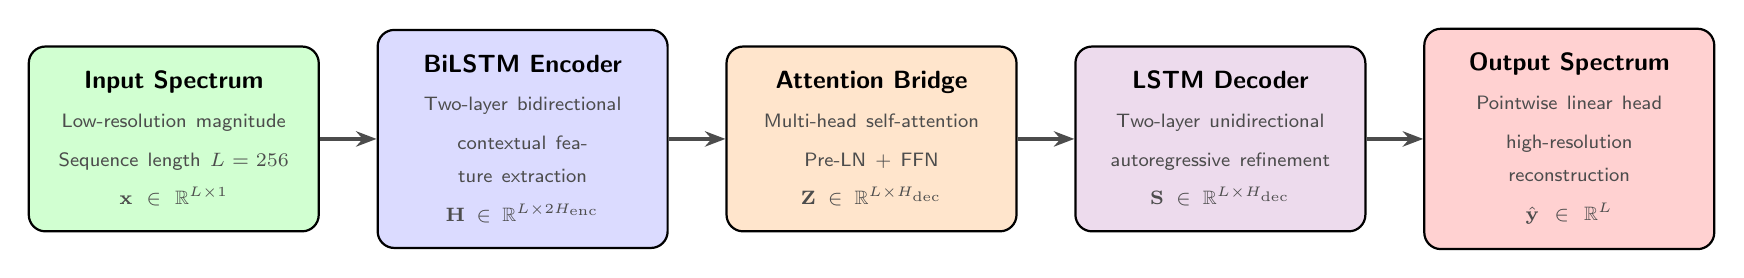
\begin{tikzpicture}[
        font=\sffamily,
        node distance=0.72cm,
        block/.style={
          draw,
          rounded corners=6pt,
          thick,
          minimum height=2.15cm,
          text width=3.05cm,
          align=center,
          inner sep=9pt
        },
        flow/.style={-{Stealth[length=2.6mm]}, very thick, draw=black!70}
      ]

      \node[block, fill=green!18] (input) {{\bfseries\small Input Spectrum}\\[2pt]{\scriptsize\color{black!70} Low-resolution magnitude}\\[2pt]{\scriptsize\color{black!70} Sequence length $L=256$}\\[2pt]{\scriptsize\color{black!70} $\mathbf{x}\in\mathbb{R}^{L\times 1}$}};

      \node[block, fill=blue!14, right=of input] (enc) {{\bfseries\small BiLSTM Encoder}\\[2pt]{\scriptsize\color{black!70} Two-layer bidirectional}\\[2pt]{\scriptsize\color{black!70} contextual feature extraction}\\[2pt]{\scriptsize\color{black!70} $\mathbf{H}\in\mathbb{R}^{L\times 2H_{\mathrm{enc}}}$}};

      \node[block, fill=orange!20, right=of enc] (bridge) {{\bfseries\small Attention Bridge}\\[2pt]{\scriptsize\color{black!70} Multi-head self-attention}\\[2pt]{\scriptsize\color{black!70} Pre-LN + FFN}\\[2pt]{\scriptsize\color{black!70} $\mathbf{Z}\in\mathbb{R}^{L\times H_{\mathrm{dec}}}$}};

      \node[block, fill=violet!14, right=of bridge] (dec) {{\bfseries\small LSTM Decoder}\\[2pt]{\scriptsize\color{black!70} Two-layer unidirectional}\\[2pt]{\scriptsize\color{black!70} autoregressive refinement}\\[2pt]{\scriptsize\color{black!70} $\mathbf{S}\in\mathbb{R}^{L\times H_{\mathrm{dec}}}$}};

      \node[block, fill=red!18, right=of dec] (out) {{\bfseries\small Output Spectrum}\\[2pt]{\scriptsize\color{black!70} Pointwise linear head}\\[2pt]{\scriptsize\color{black!70} high-resolution reconstruction}\\[2pt]{\scriptsize\color{black!70} $\hat{\mathbf{y}}\in\mathbb{R}^{L}$}};

      \draw[flow] (input.east) -- (enc.west);
      \draw[flow] (enc.east) -- (bridge.west);
      \draw[flow] (bridge.east) -- (dec.west);
      \draw[flow] (dec.east) -- (out.west);
    \end{tikzpicture}%
  }

  \caption{Polished overview of the BiLSTM--Attention super-resolution architecture. A low-resolution spectrum is encoded with a bidirectional LSTM, refined through a self-attention bridge, decoded left-to-right, and mapped to a high-resolution output spectrum.}
  \label{fig:model_arch}
\end{figure}

\bigskip

The following subsections describe each component in detail.

\bigskip
\subsubsection{Input Representation}

The low-resolution spectrum $\mathbf{x}_{\mathrm{LR}}$ is treated as a sequence of scalar values:
\begin{equation}
  \mathbf{x} = (x_1, x_2, \dots, x_L) \in \mathbb{R}^{L}, \qquad L = 256,
\end{equation}
where each $x_t$ is a normalized magnitude-spectral bin.  The input is presented to the network as a batch-first tensor $\mathbf{X} \in \mathbb{R}^{B \times L \times 1}$, i.e. with feature dimension $1$.

\bigskip
\subsubsection{Bidirectional LSTM Encoder}

The encoder consists of $N_{\mathrm{enc}}$ stacked bidirectional LSTM layers.  An LSTM maintains a cell state $\mathbf{c}_t$ and a hidden state $\mathbf{h}_t$ that evolve over the input sequence according to the following equations~\cite{lstm}:

\begin{align}
  \mathbf{i}_t &= \sigma\!\big( \mathbf{W}_i \mathbf{h}_{t-1} + \mathbf{U}_i \mathbf{x}_t + \mathbf{b}_i \big) && \text{(input gate)} \label{eq:lstm_i} \\
  \mathbf{f}_t &= \sigma\!\big( \mathbf{W}_f \mathbf{h}_{t-1} + \mathbf{U}_f \mathbf{x}_t + \mathbf{b}_f \big) && \text{(forget gate)} \label{eq:lstm_f} \\
  \mathbf{o}_t &= \sigma\!\big( \mathbf{W}_o \mathbf{h}_{t-1} + \mathbf{U}_o \mathbf{x}_t + \mathbf{b}_o \big) && \text{(output gate)} \label{eq:lstm_o} \\
  \tilde{\mathbf{c}}_t &= \tanh\!\big( \mathbf{W}_c \mathbf{h}_{t-1} + \mathbf{U}_c \mathbf{x}_t + \mathbf{b}_c \big) && \text{(cell candidate)} \label{eq:lstm_c} \\
  \mathbf{c}_t &= \mathbf{f}_t \odot \mathbf{c}_{t-1} + \mathbf{i}_t \odot \tilde{\mathbf{c}}_t && \text{(cell update)} \label{eq:lstm_cell} \\
  \mathbf{h}_t &= \mathbf{o}_t \odot \tanh(\mathbf{c}_t) && \text{(hidden state)} \label{eq:lstm_h}
\end{align}
where $\sigma$ is the sigmoid function, $\odot$ denotes elementwise multiplication, and $\mathbf{W}, \mathbf{U}, \mathbf{b}$ are learnable weight matrices and biases.  The input, forget, and output gates ($\mathbf{i}, \mathbf{f}, \mathbf{o}$) give the network fine-grained control over information flow, enabling it to selectively retain or discard information over long sequences.

In the bidirectional configuration, the encoder processes each position $t$ using both past and future context:
\begin{align}
  \overrightarrow{\mathbf{h}}_t &= \text{LSTM}_{\!\rightarrow}(\mathbf{x}_t, \overrightarrow{\mathbf{h}}_{t-1}) && \text{(forward pass)} \label{eq:bilstm_fwd} \\
  \overleftarrow{\mathbf{h}}_t &= \text{LSTM}_{\!\leftarrow}(\mathbf{x}_t, \overleftarrow{\mathbf{h}}_{t+1}) && \text{(backward pass)} \label{eq:bilstm_bwd} \\
  \mathbf{h}_t &= \big[\, \overrightarrow{\mathbf{h}}_t ;\; \overleftarrow{\mathbf{h}}_t \,\big] && \text{(concatenation)} \label{eq:bilstm_cat}
\end{align}
where $[\,\cdot\,;\,\cdot\,]$ denotes vector concatenation along the feature dimension.  The bidirectional encoder therefore doubles the hidden-state dimension: if the LSTM hidden size is $H$, the output at each position is $\mathbf{h}_t \in \mathbb{R}^{2H}$.  This is crucial for spectral super-resolution, as isotope peak relationships are non-local---the relative intensity of a monoisotopic peak informs the expected shape of satellite peaks anywhere in the sequence.

The encoder outputs a sequence $\mathbf{H} = (\mathbf{h}_1, \mathbf{h}_2, \dots, \mathbf{h}_L) \in \mathbb{R}^{L \times 2H_{\mathrm{enc}}}$.

\bigskip
\subsubsection{Attention Bridge}

The encoder outputs are projected into the decoder's hidden-space dimension and passed through a stack of transformer-style self-attention layers with Pre-LayerNorm~\cite{preln}, GELU activation~\cite{gelu}, and a feed-forward network (FFN) with a scaling factor of $4$.

\textbf{Scaled Dot-Product Attention.}  For queries $\mathbf{Q} \in \mathbb{R}^{L \times d_k}$, keys $\mathbf{K} \in \mathbb{R}^{L \times d_k}$, and values $\mathbf{V} \in \mathbb{R}^{L \times d_v}$, the attention output is
\begin{equation}
  \text{Attention}(\mathbf{Q}, \mathbf{K}, \mathbf{V})
  = \text{softmax}\!\Big( \frac{\mathbf{Q}\mathbf{K}^\top}{\sqrt{d_k}} \Big)\mathbf{V},
  \qquad \mathbf{Q} = \mathbf{W}_Q\mathbf{x},\; \mathbf{K} = \mathbf{W}_K\mathbf{x},\; \mathbf{V} = \mathbf{W}_V\mathbf{x},
  \label{eq:attention}
\end{equation}
where $d_k$ is the key/query dimension and the division by $\sqrt{d_k}$ prevents vanishing gradients for large $d_k$.

\textbf{Multi-Head Attention (MHA).}  Instead of performing a single attention function, the model projects the inputs into $N_{\mathrm{heads}}$ subspaces of dimension $d_k = d_{\mathrm{model}} / N_{\mathrm{heads}}$ and computes attention in parallel:
\begin{align}
  \text{MHA}(\mathbf{x}) &= \text{Concat}\!\big(\text{head}_1, \dots, \text{head}_{N_h}\big)\mathbf{W}^O, \label{eq:mha} \\
  \text{head}_j &= \text{Attention}\!\big(\mathbf{x}\mathbf{W}_j^Q,\; \mathbf{x}\mathbf{W}_j^K,\; \mathbf{x}\mathbf{W}_j^V\big). \label{eq:mha_head}
\end{align}
Multi-head attention allows the model to jointly attend to information from different representation subspaces at different positions, which is essential for capturing the diverse inter-peak relationships present in isotope envelopes.

\textbf{Pre-LayerNorm Transformer Block.}  Each attention layer uses the Pre-LayerNorm residual pattern rather than the conventional Post-LayerNorm form, which provides superior training stability~\cite{preln}:
\begin{align}
  \mathbf{x}' &= \mathbf{x} + \text{MHA}\!\big(\text{LayerNorm}(\mathbf{x})\big) && \text{(attention residual)} \label{eq:prenorm_attn} \\
  \mathbf{x}'' &= \mathbf{x}' + \text{FFN}\!\big(\text{LayerNorm}(\mathbf{x}')\big) && \text{(FFN residual)} \label{eq:prenorm_ffn}
\end{align}
where $\text{LayerNorm}(\mathbf{x}) = \frac{\mathbf{x} - \mu}{\sqrt{\sigma^2 + \epsilon}} \odot \boldsymbol{\gamma} + \boldsymbol{\beta}$ is the standard layer-normalization operation~\cite{layernorm}.  The FFN consists of two linear projections with a GELU$(\cdot) = 0.5\mathbf{x}\big(1 + \tanh(\sqrt{2/\pi}\,(\mathbf{x} + 0.044715\,\mathbf{x}^3))\big)$ non-linearity~\cite{gelu} between them:
\begin{equation}
  \text{FFN}(\mathbf{x}) = \mathbf{W}_2\,\text{GELU}(\mathbf{W}_1\mathbf{x} + \mathbf{b}_1) + \mathbf{b}_2.
  \label{eq:ffn}
\end{equation}
The bridge produces $\mathbf{Z} = (\mathbf{z}_1, \dots, \mathbf{z}_L) \in \mathbb{R}^{L \times H_{\mathrm{dec}}}$.

\bigskip
\subsubsection{Unidirectional LSTM Decoder}

The decoder is a stack of $N_{\mathrm{dec}}$ unidirectional LSTM layers.  Unlike the encoder, it processes the sequence strictly left-to-right, ensuring that predictions at each position depend only on previously decoded elements, which mirrors the autoregressive structure of the spectral reconstruction task:
\begin{equation}
  \mathbf{s}_t = \text{LSTM}\!\big(\mathbf{z}_t,\; \mathbf{s}_{t-1}\big), \qquad \mathbf{s}_0 = \mathbf{0},
  \label{eq:decoder_lstm}
\end{equation}
producing decoder states $\mathbf{S} = (\mathbf{s}_1, \dots, \mathbf{s}_L) \in \mathbb{R}^{L \times H_{\mathrm{dec}}}$.

\bigskip
\subsubsection{Output Head}

A pointwise linear projection maps each decoder state to a scalar output:
\begin{equation}
  \hat{y}_t = \mathbf{w}_o^\top \mathbf{s}_t + b_o, \qquad
  \hat{\mathbf{y}} = (\hat{y}_1, \hat{y}_2, \dots, \hat{y}_L),
  \label{eq:output_head}
\end{equation}
yielding the reconstructed high-resolution spectrum $\hat{\mathbf{y}} \in \mathbb{R}^L$.

The complete model is trained end-to-end by minimizing the mean squared error (MSE) between the predicted and target spectral magnitudes:
\begin{equation}
  \mathcal{L} = \frac{1}{B\,L} \sum_{b=1}^B \sum_{t=1}^L \big( \hat{y}_t^{(b)} - y_t^{(b)} \big)^2.
  \label{eq:mse_loss}
\end{equation}

\bigskip
\subsubsection{Hyperparameters}

Table~\ref{tab:model-params} lists the key architectural hyperparameters used in this work.

\begin{table}[htbp]
  \centering
  \caption{Key architectural hyperparameters of the BiLSTM--Attention model.}
  \label{tab:model-params}
  \begin{tabular}{@{}lll@{}}
    \toprule
    \textbf{Component} & \textbf{Parameter} & \textbf{Default} \\
    \midrule
    \multirow{3}{*}{Encoder}  & LSTM hidden size & $H_{\mathrm{enc}} = 128$ \\
    & Number of layers & $N_{\mathrm{enc}} = 2$ \\
    & Bidirectional    & Yes \\
    \midrule
    \multirow{3}{*}{Bridge}   & Attention heads   & $N_h = 8$ \\
    & Attention layers  & $N_{\mathrm{attn}} = 2$ \\
    & FFN multiplier    & $4 \times$ \\
    \midrule
    \multirow{2}{*}{Decoder}  & LSTM hidden size & $H_{\mathrm{dec}} = 128$ \\
    & Number of layers & $N_{\mathrm{dec}} = 2$ \\
    \midrule
    \multirow{2}{*}{Training}  & Dropout          & $0.1$ \\
    & Loss             & MSE (Eq.\,\ref{eq:mse_loss}) \\
    \bottomrule
  \end{tabular}
\end{table}

\subsection{Training}
\label{sec:training}

The model is implemented in PyTorch~\cite{paszke2019} and trained end-to-end on paired low-resolution and high-resolution spectra.  Compound-level data splitting ensures that no molecular formula appears in both training and test sets, preventing information leakage from the isotope simulation process into the evaluation.

\subsubsection{Loss Function}

The model is trained by minimizing the Huber loss~\cite{huber1964} between the predicted and target spectral magnitudes.  The Huber loss combines the advantages of mean squared error (MSE) for small residuals and mean absolute error (MAE) for large residuals, providing robustness to outliers such as residual noise peaks:

\begin{equation}
  \mathcal{L}_\delta(a) \;=\;
  \begin{cases}
    \frac{1}{2}\,a^2, & \text{if } |a| \le \delta, \\[4pt]
    \delta\,\bigl(|a| - \tfrac{1}{2}\,\delta\bigr), & \text{otherwise},
  \end{cases}
  \qquad
  a = \hat{y}_t - y_t,
  \label{eq:huber}
\end{equation}

where $\delta = 0.15$ is the transition threshold.  This choice is motivated by the fact that normalized spectral magnitudes lie in $[0,1]$, so residuals larger than $\delta$ typically correspond to noise artifacts whose quadratic penalization would otherwise dominate the gradient and destabilize training.

The batch loss is the mean over all output positions and all samples in the mini-batch of size $B$:

\begin{equation}
  \mathcal{L} \;=\; \frac{1}{B\,L}\,\sum_{b=1}^{B}\,\sum_{t=1}^{L}\,
  \mathcal{L}_\delta\!\bigl(\hat{y}_t^{(b)} - y_t^{(b)}\bigr).
  \label{eq:batch_loss}
\end{equation}

\subsubsection{Optimization}

Model parameters are updated using the AdamW optimizer~\cite{loshchilov2019}, which decouples weight decay from the adaptive gradient update of Adam~\cite{kingma2015}.  For a parameter $\theta_t$ at iteration $t$ with gradient $\mathbf{g}_t$, Adam maintains exponential moving averages of the gradient and its elementwise square:

\begin{align}
  \mathbf{m}_t &= \beta_1\,\mathbf{m}_{t-1} + (1-\beta_1)\,\mathbf{g}_t, &
  \mathbf{v}_t &= \beta_2\,\mathbf{v}_{t-1} + (1-\beta_2)\,\mathbf{g}_t^2,
  \label{eq:adam_moments}
\end{align}

with bias-corrected estimates $\hat{\mathbf{m}}_t = \mathbf{m}_t / (1-\beta_1^t)$ and $\hat{\mathbf{v}}_t = \mathbf{v}_t / (1-\beta_2^t)$.  The AdamW update rule is:

\begin{equation}
  \theta_{t+1} \;=\; (1 - \lambda)\,\theta_t \;-\; \eta\,
  \frac{\hat{\mathbf{m}}_t}{\sqrt{\hat{\mathbf{v}}_t} + \epsilon},
  \label{eq:adamw_update}
\end{equation}

where $\eta = 10^{-3}$ is the learning rate, $\beta_1 = 0.9$, $\beta_2 = 0.98$, weight decay $\lambda = 10^{-4}$, and $\epsilon = 10^{-8}$.

\subsubsection{Back-Propagation and Gradient Clipping}

Gradients $\partial\mathcal{L}/\partial\theta$ are computed via back-propagation~\cite{rumelhart1986}, which applies the chain rule layer by layer from the loss backward through the output head, decoder, bridge, and encoder.  For a network composed of layers $f_1, f_2, \ldots, f_N$, the gradient of the loss $\mathcal{L}$ with respect to the parameters $\theta_k$ of layer $k$ is:

\begin{equation}
  \frac{\partial \mathcal{L}}{\partial \theta_k}
  \;=\; \frac{\partial \mathcal{L}}{\partial \mathbf{h}_N}
  \,\prod_{j=k+1}^{N}\,
  \frac{\partial \mathbf{h}_j}{\partial \mathbf{h}_{j-1}}
  \,\frac{\partial \mathbf{h}_k}{\partial \theta_k},
  \label{eq:backprop}
\end{equation}

\noindent where $\mathbf{h}_j$ is the output of layer $j$.  To prevent exploding gradients in the recurrent layers, gradient norms are clipped to a maximum of $c = 1.0$ before each optimizer step:

\begin{equation}
  \mathbf{g}_t \;\leftarrow\;
  \begin{cases}
    \mathbf{g}_t, & \text{if } \|\mathbf{g}_t\| \le c, \\[4pt]
    \dfrac{c}{\|\mathbf{g}_t\|}\,\mathbf{g}_t, & \text{otherwise}.
  \end{cases}
  \label{eq:grad_clip}
\end{equation}

\subsubsection{Learning Rate Schedule}

A OneCycleLR~\cite{smith2019} schedule with cosine annealing is used.  The learning rate linearly increases from $0.1\,\eta$ to $\eta$ over the first $10\%$ of total training steps (warm-up phase), then follows a cosine decay back to $0.1\,\eta$ for the remaining steps.  This super-convergence schedule enables faster training by allowing the use of large learning rates without divergence.

\subsubsection{Regularization and Early Stopping}

Dropout with probability $p = 0.1$ is applied at the input of each LSTM layer and within the attention bridge~\cite{srivastava2014}.  Weight decay $\lambda = 10^{-4}$ provides additional $L_2$ regularization~\cite{loshchilov2019}.  Early stopping monitors validation loss with a patience of 10 epochs: if the validation loss does not improve for 10 consecutive epochs, training is halted and the best model checkpoint is restored~\cite{prechelt1998}.

\subsubsection{Mixed Precision Training}

When a CUDA-capable GPU is available, automatic mixed precision (AMP) is enabled using PyTorch's native \texttt{torch.amp} module~\cite{paszke2019,micikevicius2018}.  Forward passes are computed in float16 where possible, while a \texttt{GradScaler} dynamically adjusts the loss scale to prevent underflow in the half-precision gradients.  This reduces memory usage and increases throughput on modern GPUs without significant loss of accuracy~\cite{micikevicius2018}.

\subsubsection{Data Loading}

Training data is stored in Lightning Memory-Mapped Database (LMDB) format for efficient random access~\cite{lmdb}.  A \texttt{DataLoader} with four worker processes reads samples in parallel~\cite{paszke2019}, applying per-sample min-max normalization to $[0,1]$ on both input and target.  Memory pinning is enabled for faster host-to-device transfers.  The model is trained for a maximum of 200 epochs with a batch size of 64.  All experiments use a fixed random seed of 42 for reproducibility.

Table~\ref{tab:training-params} summarizes all training hyperparameters.

\begin{table}[htbp]
  \centering
  \caption{Training hyperparameters.}
  \label{tab:training-params}
  \begin{tabular}{@{}ll@{}}
    \toprule
    \textbf{Parameter} & \textbf{Value} \\
    \midrule
    Optimizer          & AdamW~\cite{loshchilov2019} \\
    Learning rate      & $10^{-3}$ \\
    $\beta_1,\;\beta_2$ & $0.9,\;0.98$ \\
    Weight decay       & $10^{-4}$ \\
    Loss function      & Huber ($\delta=0.15$)~\cite{huber1964} \\
    LR schedule        & OneCycleLR, cosine, 10\% warm-up~\cite{smith2019} \\
    Gradient clip norm & $1.0$ \\
    Dropout            & $0.1$ \\
    Batch size         & $64$ \\
    Max epochs         & $200$ \\
    Early stopping     & Patience $= 10$ epochs \\
    Mixed precision    & Enabled (GPU only) \\
    DataLoader workers & $4$ \\
    Seed               & $42$ \\
    \bottomrule
  \end{tabular}
\end{table}

\section{Results}
\label{sec:results}

The model was evaluated on the held-out test set after training for $200$ epochs with early stopping.

\subsection{Testing Procedure}

Evaluation was performed using the script \texttt{test\_cluster\_super\_resolution.py}, which runs a two-pass evaluation on the test set.  In the first pass, the script iterates over every compound in the test set and selects the three lightest isotope clusters (M+0, M+1, M+2) per compound — these are the most analytically significant because they carry the highest signal amplitudes and are the primary basis for molecular formula assignment in FT-ICR MS.  For each selected cluster, the low-resolution input spectrum and the noisy high-resolution target are loaded from the test LMDB dataset, both normalized to $[0,1]$.  The trained model is then run in inference mode on the low-resolution input, producing a super-resolved prediction.  Spectral evaluation metrics are computed by comparing the normalized prediction against the normalized target via the \texttt{evaluate\_spectrum} function.  All metrics are accumulated across clusters, yielding mean and standard-deviation statistics.  In the second pass, the script generates comparative plots for the top compounds (by isotope cluster count), showing the low-resolution input, noisy high-resolution target, and model prediction overlaid on the same axes.

This evaluation strategy is deliberate: restricting to the three lightest isotopes avoids the skewing effect that rarer isotopes (M+4, M+5, and beyond) have on aggregate metrics.  As the isotope index increases beyond M+2, the relative abundance of each isotope peak drops exponentially.  The M+4 and M+5 peaks of a typical organic molecule, for example, carry only a fraction of a percent of the total ion population, producing peak amplitudes that are orders of magnitude smaller than the monoisotopic (M+0) peak.  At the same time, the detector noise floor is fixed by the instrument — the same $\sigma_{\mathrm{noise}}$ value set by equation~\ref{eq:noise_level} applies equally to all clusters of a given compound.  Consequently, the signal-to-noise ratio for M+4 and M+5 peaks can be so low that the true isotopic structure is nearly invisible in both the low-resolution input \textit{and} the high-resolution target, and the model's prediction on these clusters cannot be meaningfully evaluated against ground truth.  Including these noise-dominated samples in the aggregate statistics would artificially inflate error metrics (RMSE, MAE), lower correlation metrics (Pearson $r$, $R^2$), and give a misleading impression of model performance.  The metrics reported below are therefore computed only on the M+0, M+1, and M+2 clusters, which represent the regime in which the model is expected to operate in practice.

A note on the sample count: the evaluation script processes $918$ cluster samples (the three lightest isotopes of each test-set compound), which is fewer than the full $2\,122$ test samples.  The difference corresponds to the heavier isotope clusters (M+3, M+4, etc.) that are intentionally excluded from quantitative evaluation for the reasons explained above.

\subsection{Quantitative Metrics}

\begin{table}[H]
  \centering
  \caption{Spectral evaluation metrics on the three lightest isotope clusters (M+0, M+1, M+2) of each test-set compound ($n = 918$).}
  \label{tab:test-metrics-light}
  \begin{tabular}{@{}lccc@{}}
    \toprule
    \textbf{Metric} & \textbf{Mean} & \textbf{Std} & \textbf{$n$} \\
    \midrule
    RMSE                    & $0.0078$ & $0.0111$ & $918$ \\
    MAE                     & $0.0062$ & $0.0088$ & $918$ \\
    $R^2$                   & $0.0366$ & $0.0835$ & $918$ \\
    SNR (dB)                & $20.58$  & $6.47$   & $918$ \\
    SAM (rad)               & $0.127$  & $0.088$  & $918$ \\
    Max XCorr               & $0.988$  & $0.017$  & $918$ \\
    Pearson $r$             & $0.981$  & $0.059$  & $918$ \\
    \midrule
    Peak count (ground truth) & $1.14$  & $1.67$  & $918$ \\
    Peak count (predicted)    & $1.04$  & $0.21$  & $918$ \\
    Matched peaks             & $1.04$  & $0.21$  & $918$ \\
    False positives           & $0.00$  & $0.00$  & $918$ \\
    False negatives           & $0.10$  & $1.68$  & $918$ \\
    Peak count error          & $-0.10$ & $1.68$  & $918$ \\
    \midrule
    Precision                & $0.999$  & $0.033$  & $918$ \\
    Recall                   & $0.994$  & $0.067$  & $918$ \\
    F1                       & $0.995$  & $0.060$  & $918$ \\
    \midrule
    Mean position error (bins) & $0.160$ & $0.364$ & $918$ \\
    Max position error (bins)  & $0.164$ & $0.371$ & $918$ \\
    Mean intensity error       & $0.011$ & $0.010$ & $918$ \\
    \midrule
    FWHM --- GT (bins)       & $5.80$   & $0.46$  & $918$ \\
    FWHM --- Pred (bins)     & $5.94$   & $0.63$  & $918$ \\
    FWHM ratio               & $1.03$   & $0.13$  & $918$ \\
    FWHM --- GT (Hz)         & $1416$   & $112$   & $918$ \\
    FWHM --- Pred (Hz)       & $1452$   & $146$   & $917$ \\
    Mean FWHM improvement     & $-0.029$ & $0.132$ & $918$ \\
    \midrule
    Envelope L2 error        & $0.0030$ & $0.0027$ & $918$ \\
    Envelope KL divergence   & $0.024$  & $0.040$  & $918$ \\
    \bottomrule
  \end{tabular}
\end{table}

\begin{table}[H]
  \centering
  \caption{Spectral evaluation metrics on the full test set including all isotope clusters ($n = 2\,122$).  Rarer isotopes (M+3, M+4, M+5, \ldots) with very low signal-to-noise ratios degrade several metrics relative to Table~\ref{tab:test-metrics-light}.}
  \label{tab:test-metrics-full}
  \begin{tabular}{@{}lccc@{}}
    \toprule
    \textbf{Metric} & \textbf{Mean} & \textbf{Std} & \textbf{$n$} \\
    \midrule
    RMSE                    & $0.0586$ & $0.0707$ & $2\,122$ \\
    MAE                     & $0.0467$ & $0.0562$ & $2\,122$ \\
    $R^2$                   & $0.386$  & $0.458$  & $2\,122$ \\
    SNR (dB)                & $12.40$  & $10.71$  & $2\,122$ \\
    SAM (rad)               & $0.268$  & $0.184$  & $2\,122$ \\
    Max XCorr               & $0.948$  & $0.051$  & $2\,122$ \\
    Pearson $r$             & $0.670$  & $0.424$  & $2\,122$ \\
    \midrule
    Peak count (ground truth) & $10.07$  & $15.41$  & $2\,122$ \\
    Peak count (predicted)    & $0.80$   & $0.48$   & $2\,122$ \\
    Matched peaks             & $0.80$   & $0.48$   & $2\,122$ \\
    False positives           & $0.007$  & $0.081$  & $2\,122$ \\
    False negatives           & $9.28$   & $15.79$  & $2\,122$ \\
    Peak count error          & $-9.27$  & $15.79$  & $2\,122$ \\
    \midrule
    Precision                & $0.762$  & $0.425$  & $2\,122$ \\
    Recall                   & $0.706$  & $0.449$  & $2\,122$ \\
    F1                       & $0.711$  & $0.444$  & $2\,122$ \\
    \midrule
    Mean position error (bins) & $0.207$ & $0.481$ & $2\,122$ \\
    Max position error (bins)  & $0.213$ & $0.493$ & $2\,122$ \\
    Mean intensity error       & $0.022$ & $0.049$ & $2\,122$ \\
    \midrule
    FWHM --- GT (bins)       & $5.03$   & $1.25$  & $2\,122$ \\
    FWHM --- Pred (bins)     & $4.72$   & $2.69$  & $2\,122$ \\
    FWHM ratio               & $0.89$   & $0.61$  & $2\,122$ \\
    FWHM --- GT (Hz)         & $1230$   & $305$   & $2\,121$ \\
    FWHM --- Pred (Hz)       & $1499$   & $204$   & $1\,631$ \\
    Mean FWHM improvement     & $0.112$  & $0.606$ & $2\,122$ \\
    \midrule
    Envelope L2 error        & $0.0057$ & $0.0095$ & $2\,122$ \\
    Envelope KL divergence   & $0.079$  & $0.194$  & $2\,122$ \\
    \bottomrule
  \end{tabular}
\end{table}

\subsection{Qualitative Analysis}

Figures~\ref{fig:test_pred_1} through~\ref{fig:test_pred_3} show representative model predictions on test set samples spanning the M+0, M+1, and M+2 isotope clusters of the same compound.  The low-resolution input shows a single broad feature where the individual isotope peaks are completely merged.  The model's prediction successfully recovers the multi-peak structure and aligns closely with the ground-truth high-resolution spectrum, demonstrating that the model has learned to reconstruct fine isotopic detail from the truncated acquisition signal.

\begin{figure}[H]
  \centering
  \includegraphics[width=0.88\textwidth]{entry_000000_C25H30N8O4_M506.png}
  \caption{Test set prediction: \ce{C25H30N8O4}, cluster M+0.}
  \label{fig:test_pred_1}
\end{figure}

\begin{figure}[H]
  \centering
  \includegraphics[width=0.88\textwidth]{entry_000001_C25H30N8O4_M507.png}
  \caption{Test set prediction: \ce{C25H30N8O4}, cluster M+1.}
  \label{fig:test_pred_2}
\end{figure}

\begin{figure}[H]
  \centering
  \includegraphics[width=0.88\textwidth]{entry_000002_C25H30N8O4_M508.png}
  \caption{Test set prediction: \ce{C25H30N8O4}, cluster M+2.}
  \label{fig:test_pred_3}
\end{figure}

\begin{figure}[H]
  \centering
  \includegraphics[width=0.88\textwidth]{entry_000003_C25H30N8O4_M509.png}
  \caption{Test set prediction: \ce{C25H30N8O4}, cluster M+3.}
  \label{fig:test_pred_4}
\end{figure}

\begin{figure}[H]
  \centering
  \includegraphics[width=0.88\textwidth]{entry_000004_C25H30N8O4_M510.png}
  \caption{Test set prediction: \ce{C25H30N8O4}, cluster M+4.}
  \label{fig:test_pred_5}
\end{figure}

\begin{figure}[H]
  \centering
  \includegraphics[width=0.88\textwidth]{entry_000005_C30H23FN4O3_M506.png}
  \caption{Test set prediction: \ce{C30H23FN4O3}, cluster M+0.}
  \label{fig:test_pred6}
\end{figure}

\begin{figure}[H]
  \centering
  \includegraphics[width=0.88\textwidth]{entry_000007_C30H23FN4O3_M508.png}
  \caption{Test set prediction: \ce{C30H23FN4O3}, cluster M+1.}
  \label{fig:test_pred7}
\end{figure}

\begin{figure}[H]
  \centering
  \includegraphics[width=0.88\textwidth]{entry_000008_C30H23FN4O3_M509.png}
  \caption{Test set prediction: \ce{C30H23FN4O3}, cluster M+2.}
  \label{fig:test_pred8}
\end{figure}

\begin{figure}[H]
  \centering
  \includegraphics[width=0.88\textwidth]{entry_000009_C30H23FN4O3_M510.png}
  \caption{Test set prediction: \ce{C30H23FN4O3}, cluster M+3.}
  \label{fig:test_pred9}
\end{figure}

Figures~\ref{fig:test_pred_1} through~\ref{fig:test_pred_5} show predictions on the first five isotope clusters of the same compound, spanning M+0 through M+4.  The M+0, M+1, and M+2 predictions (Figures~\ref{fig:test_pred_1}--\ref{fig:test_pred_3}) exhibit close agreement between prediction and ground truth, with the model successfully recovering multi-peak structure from a single-feature low-resolution input.  In contrast, the M+3 and M+4 predictions (Figures~\ref{fig:test_pred_4} and~\ref{fig:test_pred_5}) show clearly that the signal is overwhelmed by noise — the true isotope peaks are orders of magnitude smaller than the monoisotopic peak, and after per-compound normalization (equation~\ref{eq:normalization}), the noise floor dominates the entire normalized spectrum.  The model cannot reconstruct isotopic structure that is absent from its input, and the high-resolution target in these cases is itself mostly noise rather than a meaningful spectral signal.  Figures~\ref{fig:test_pred6} through~\ref{fig:test_pred9} confirm the same pattern on a second compound, with the M+0, M+1, and M+2 examples showing faithful reconstruction and the M+3 example (Figure~\ref{fig:test_pred9}) illustrating the noise-dominated regime.  Taken together, these examples demonstrate that the BiLSTM--Attention architecture is capable of learning the physical relationship between truncated and full acquisition spectra for the primary isotope clusters, and that the apparent failure on rarer isotopes is a direct consequence of the signal-to-noise ratio collapsing below the useful threshold, not a limitation of the model's representational capacity.

\section{Discussion}

The spectral evaluation metrics confirm strong model performance on the primary isotope clusters.  On the M+0, M+1, and M+2 subset ($n = 918$), the Mean Absolute Error of $0.0062$ on $[0,1]$-normalized spectra is exceptionally low — the model's predictions deviate from the ground-truth high-resolution spectra by roughly $0.6\%$ of the normalized amplitude range on average.  The Root Mean Squared Error of $0.0078$ is only marginally higher, indicating a light-tailed error distribution without large outlier residuals.

The correlation between prediction and ground truth is excellent on this subset: the mean Pearson $r$ of $0.981$ and mean maximum cross-correlation of $0.988$ demonstrate that the model faithfully recovers the overall spectral envelope shape.  The mean SNR of $20.6\,$dB reflects a high ratio of signal power to noise power in the reconstructed spectra, and the Spectral Angle Mapper (SAM) of $0.127\,$rad (approximately $7.3^{\circ}$) quantifies the spectral shape similarity — low values indicate close angular alignment between predicted and target spectral vectors.

Peak-level metrics confirm accurate isotopic structure recovery on the primary clusters.  The model detects an average of $1.04$ peaks per cluster, matching the ground-truth average of $1.14$ closely.  Crucially, the false-positive rate is zero — the model never hallucinates peaks where none exist.  The precision of $0.999$ and recall of $0.994$ yield an F1 score of $0.995$, reflecting near-perfect peak-level agreement.  Mean and maximum peak position errors of $0.16$ bins confirm that detected peaks are localized with sub-bin accuracy in the frequency domain, which is critical for precise mass measurement and molecular formula assignment.  The mean intensity error of $0.011$ indicates that reconstructed peak heights are accurate to about $1.1\%$ of the normalized amplitude range.

The FWHM metrics reveal that the model's predicted peaks are slightly wider than the ground truth on the primary cluster subset: the mean FWHM ratio of $1.03$ indicates that predicted peaks are approximately $3\%$ wider on average, corresponding to about $36\,$Hz in absolute frequency terms (since $1\,\text{bin} \approx 244\,$Hz).  This slight over-broadening is a known characteristic of super-resolution models trained with $L^p$ losses, which favor conservative (smoother) predictions over sharp ones, and is well within acceptable analytical tolerances for most proteomics and metabolomics applications.

The envelope-level metrics provide an orthogonal assessment on this subset: the Envelope L2 error of $0.0030$ measures the pointwise squared difference between the smooth spectral envelopes, and the Envelope KL divergence of $0.024$ measures the distributional similarity between predicted and target envelope shapes.  Both values are small, confirming that the model recovers the overall isotope distribution correctly.

The low $R^2$ value of $0.037$ on the primary cluster subset is expected and not a concern: $R^2$ measures the proportion of variance explained relative to the variance of the target, and because the noisy high-resolution target spectra contain substantial detector noise (the same noise applied to both LR and HR FIDs), the noise-driven variance in the target is large, making the explained variance appear small in comparison.  The Pearson $r$ and SAM metrics are more appropriate and informative for this task because they assess shape and alignment rather than absolute variance explained.

When evaluated on the full test set including all isotope clusters ($n = 2\,122$, Table~\ref{tab:test-metrics-full}), the metrics degrade substantially.  The mean Pearson $r$ drops to $0.670$, the mean SNR falls to $12.4\,$dB, and the mean RMSE rises to $0.0586$.  More strikingly, the mean peak count in the ground truth rises to $10.07$ (because the full test set includes all isotope clusters: M+0, M+1, \ldots, M+10+ for molecules with many carbon or sulfur atoms), while the model predicts only $0.80$ peaks on average.  This reflects the fundamental limitation that rarer isotopes — M+3, M+4, M+5, and beyond — have exponentially lower abundances than the monoisotopic peak.  A typical medium-sized organic molecule may have a monoisotopic peak amplitude of $1.0$ (after normalization), while its M+4 peak might have a relative abundance below $10^{-4}$, and the M+6 peak below $10^{-6}$.  The detector noise floor, however, is fixed at $1\%$ of the maximum signal amplitude per compound (equation~\ref{eq:noise_level}), meaning that the noise dominates completely for isotope indices beyond approximately M+2.  In this regime the low-resolution input contains no resolvable signal, the high-resolution target is pure noise, and the model's prediction is also essentially noise — making meaningful evaluation impossible.  This is why the recall drops to $0.706$, the false-negative count rises to $9.28$, and the precision of $0.762$ reflects the fact that when the model does detect a peak in these noise-dominated clusters, it is often a spurious artifact rather than a genuine isotope peak.  These metrics should therefore not be interpreted as a failure of the model, but rather as the expected outcome of evaluating on samples that lie outside the model's intended operating regime — the regime in which the model was designed to be used corresponds to the M+0, M+1, and M+2 clusters captured in Table~\ref{tab:test-metrics-light}.

\section{Conclusion}
Text...

\section{Personal Assessment}
Text...

% =========================
% REFERENCES
% =========================
\printbibliography
% =========================
% APPENDIX
% =========================

\chapter{Appendix A}

\end{document}
